\documentclass{article}
% General
	\usepackage{graphicx} % Required for inserting images
	\setlength{\parindent}{0pt}
	\setlength{\parskip}{8pt} % Vertical space between paragraphs
	\setlength{\baselineskip}{18pt} % Vertical space between lines
	\usepackage{amsthm}
	\usepackage{mdframed}
	\usepackage{hyperref} % Add the hyperref package for clickable links
	\newcommand\bigO{\mathrm{O}}
	\usepackage[T1]{fontenc}
	\usepackage{amsfonts}

% Define the theorem-like environments
	% Define a new theorem style with upright text
	\newtheoremstyle{plainupright} % Name of the style
	{10pt}                        % Space above
	{3pt}                        % Space below
	{}                           % Body font (default is \itshape which is italics)
	{}                           % Indent amount
	{\bfseries}                  % Theorem head font
	{.}                          % Punctuation after theorem head
	{ }                          % Space after theorem head
	{}                           % Theorem head spec (can be left empty, meaning 'normal')
	
	\theoremstyle{plainupright}

	\newtheorem{theorem}{Theorem}[section]  % Numbering within sections
	\newtheorem{definition}[theorem]{Definition}  % Numbering with theorems
	\newtheorem{corollary}[theorem]{Corollary}  % Numbering with theorems
	\newtheorem{claim}[theorem]{Claim}  % Numbering with theorems
	\newtheorem{lemma}[theorem]{Lemma}  % Numbering with theorems
	\newtheorem{axiom}[theorem]{Axiom}  % Numbering with theorems
	\newtheorem{conjecture}[theorem]{Conjecture}  % Numbering with theorems
	\newtheorem{problem}[theorem]{Problem}  % Numbering with theorems

% Enclose theorem-like environments within boxes
	\surroundwithmdframed[style=theoremstyle]{theorem}
	\surroundwithmdframed[style=theoremstyle]{definition}
	\surroundwithmdframed[style=theoremstyle]{corollary}
	\surroundwithmdframed[style=theoremstyle]{claim}
	\surroundwithmdframed[style=theoremstyle]{lemma}
	\surroundwithmdframed[style=theoremstyle]{axiom}
	\surroundwithmdframed[style=theoremstyle]{conjecture}
	\surroundwithmdframed[style=theoremstyle]{problem}

% Define a box style for the theorem-like environments
	\mdfdefinestyle{theoremstyle}{%
		linewidth=0pt,
		backgroundcolor=white,
		roundcorner=5pt,
		innertopmargin=6pt,
		innerbottommargin=0pt,
		innerrightmargin=32pt,
		innerleftmargin=16pt,
	}	

% Set margins
	\usepackage{geometry}
	\geometry{
		left=3cm,
		right=3cm,
		top=2cm,
		bottom=2cm
	}

% Codeblock
	\usepackage{minted}
	\usepackage{xcolor}
	\definecolor{mintedBg}{rgb}{0.98,0.98,0.98}
	\setminted[py]{
		bgcolor=mintedBg,
		framesep=3mm,
		fontsize=\footnotesize,
		linenos,
		breaklines,
		breakanywhere,
	}
	\newcommand{\pyfile}[3]{%
		\textsf{%
			\detokenize{#1}%
		}%
		\par
		\inputminted[firstline=#2,lastline=#3]{py}{../code/\detokenize{#1}}%
	}

\newcommand{\todo}[1]{\textcolor{red}{#1}}



\title{Implementation of a minimal branch-decomposition algorithm for planar graphs.}
\author{Kristoffer Højelse}
\date{February 2024}

\begin{document}

\maketitle

% west https://dwest.web.illinois.edu/grammar.html
% The abstract states the results as fully as possible in a brief presentation. Crucial specialized terms the reader needs to know to understand the statements should be defined. The abstract stands on its own, especially in the age of electronic communication where it may be separate from the rest of the paper, and hence it contains no numbered reference to the bibliography.

\begin{abstract}
	Seymour and Thomas give an algorithm, the rat-catching algorithm, for deciding $bw(G) \leq c$ in $O(n^2)$ time, and by using it as a subroutine, an algorithm to compute an optimal branch-decomposition in $O(n^4)$ time. In this paper, I describe an implementation of this algorithm and publish the source code.
\end{abstract}

% The first section of the paper is an "Introduction" that should motivate the problem, discuss related results, state the results more completely, and perhaps summarize the techniques or the structure of the paper or crucial definitions.

\section{Introduction}
	Some graph optimization problems can be solved efficiently for graphs of small branchwidth.\cite{CNP+11}

	Pino\cite{Pin16} applies branch decompositions.

	Seymour and Thomas\cite{ST93} give the rat-catching algorithm.

	Bian, Gu and Zhu\cite{BGZ15} describe and benchmark some implementations.

	\todo{which? counting Hamiltonian cycles of planar cubic graphs}

\section{Preliminaries}

	A \textit{graph} $G$ consists of a vertex set $V(G)$, and an edge set $\mathbb{E}(G)$ and a function $\phi_G$, where $V(G) \subset \mathbb{N}^+$ and where $\mathbb{E}(G) \subset \mathbb{N}^+$ and where $\phi_G \st \mathbb{E}(G) \to \{\{u,v\} \st u,v \in V(G)\}$.
	
	\textbf{Note.} Other authors might instead call this definition an undirected labelled pseudograph, with edges having own identity.
	
	\textbf{Note.} Regarding notation, $V$ and $\mathbb{E}$ are operations on graphs returning the vertex set and edge set respectively.

	A \textit{drawing} of a graph $G$ is a node-link diagram in which the vertices are represented as disks and the edges are represented as line segments or curves in the Euclidean plane.

	Here is a drawing of a graph $G$.

	\begin{center}
		\input{images/unlabeled-graph.tex}
	\end{center}

	Here is a labeled drawing of the same graph $G$ and its function $\phi_G$.

	\begin{center}
		\input{images/graph.tex}
	\end{center}

	Let $E(G)$ return a multiset of all vertex-pairs of $G$; in other words, $E(G) = \{\phi_G(e) \st e \in \mathbb{E}(G)\}$.

	A edge $e$ where $\phi_G(e) = \{u,v\}$, is a \textit{self-loop}, if $u = v$.

	A graph $G$ is \textit{loop-less}, if no edge $e \in \mathbb{E}(G)$ is a self-loop.

	A \textit{multi-graph} is a graph that is loop-less.

	\begin{center}
		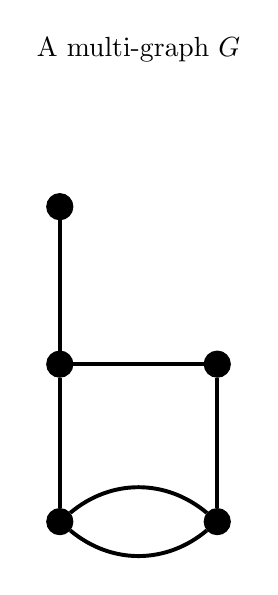
\begin{tikzpicture}
    % Define the nodes with specific positions
    \begin{scope}[xshift=0cm, yshift=0cm]
        \node (G) at (1, 6) {A multi-graph $G$};

        \node[circle, draw, fill=black, minimum size=0.01mm] (1) at (0, 4) {};
        \node[circle, draw, fill=black, minimum size=0.01mm] (2) at (0, 2) {};
        \node[circle, draw, fill=black, minimum size=0.01mm] (3) at (0, 0) {};
        \node[circle, draw, fill=black, minimum size=0.01mm] (4) at (2, 2) {};
        \node[circle, draw, fill=black, minimum size=0.01mm] (5) at (2, 0) {};

        % Draw the edges between nodes
        \draw[line width=0.5mm] (1) -- (2);
        \draw[line width=0.5mm] (2) -- (3);
        \draw[line width=0.5mm] (2) -- (4);
        \draw[line width=0.5mm] (4) -- (5);
        \draw[line width=0.5mm] (3) to[bend left=40] (5);
        \draw[line width=0.5mm] (3) to[bend right=40] (5);
    \end{scope}
\end{tikzpicture}

	\end{center}

	A multi-graph $G$ is \textit{simple}, if it has no parallel edges; in other words, if elements of $E(G)$ are pair-wise distinct.

	\begin{center}
		\input{images/simple-graph.tex}
	\end{center}

	A \textit{subgraph} $H$ of a graph $G$, is a graph where some vertices and edges might be missing; in other words, is a graph where $V(H) \subseteq V(G)$ and where $\mathbb{E}(H) \subseteq \mathbb{E}(G)$ and where $\forall e \in \mathbb{E}(H), \phi_H(e) = \phi_G(e)$.

	\begin{center}
		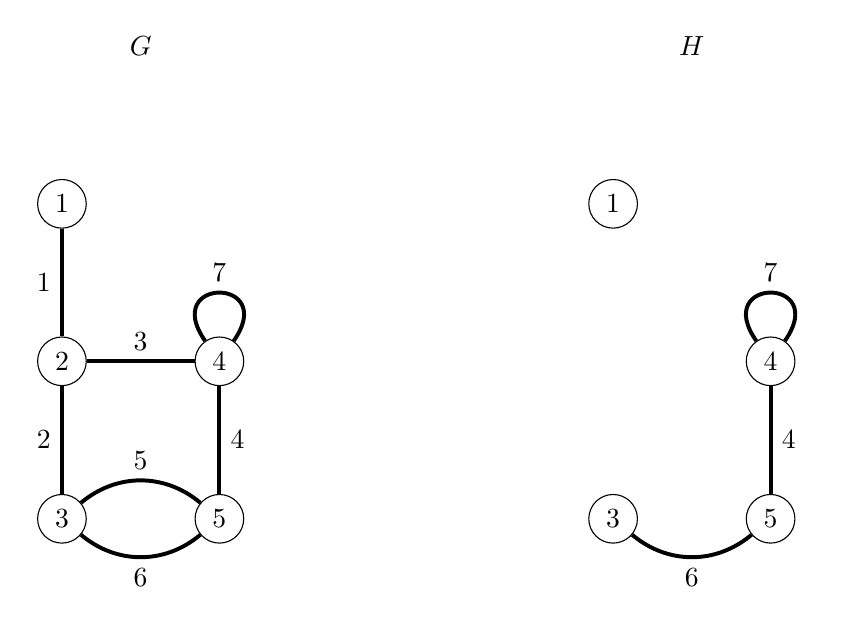
\begin{tikzpicture}
	\begin{scope}[xshift=0cm, yshift=0cm]
		\node (G) at (1, 6) {$G$};

		\node[circle, draw] (1) at (0, 4) {1};
		\node[circle, draw] (2) at (0, 2) {2};
		\node[circle, draw] (3) at (0, 0) {3};
		\node[circle, draw] (4) at (2, 2) {4};
		\node[circle, draw] (5) at (2, 0) {5};
	
		% Draw the edges between nodes with labels
		\draw[line width=0.5mm] (1) -- node[left] {1} (2);
		\draw[line width=0.5mm] (2) -- node[left] {2} (3);
		\draw[line width=0.5mm] (2) -- node[above] {3} (4);
		\draw[line width=0.5mm] (4) -- node[right] {4} (5);
		\draw[line width=0.5mm] (3) to[bend left=40] node[above] {5} (5);
		\draw[line width=0.5mm] (3) to[bend right=40] node[below] {6} (5);
		\draw[line width=0.5mm] (4) to[in=125,out=55,loop, min distance=1cm] node[above] {7} (4);
	\end{scope}

	\begin{scope}[xshift=7cm, yshift=0cm]
		\node (G) at (1, 6) {$H$};

		\node[circle, draw] (1) at (0, 4) {1};
		\node[circle, draw] (3) at (0, 0) {3};
		\node[circle, draw] (4) at (2, 2) {4};
		\node[circle, draw] (5) at (2, 0) {5};
	
		% Draw the edges between nodes with labels
		\draw[line width=0.5mm] (4) -- node[right] {4} (5);
		\draw[line width=0.5mm] (3) to[bend right=40] node[below] {6} (5);
		\draw[line width=0.5mm] (4) to[in=125,out=55,loop, min distance=1cm] node[above] {7} (4);
	\end{scope}
\end{tikzpicture}

	\end{center}

	For $A \subseteq V(G)$, we denote by $G[A]$ the subgraph induced by the subset of vertices $A$; in other words, $G[A]$ is the subgraph where $V(G[A]) = A$ and where $\mathbb{E}(G[A]) = \{ e \st e \in \mathbb{E}(G) \land |\phi_G(e) \cap A| = 2\}$ and where $\forall e \in E(G[A]), \phi_{G[A]}(e) = \phi_{G}(e)$.

	\begin{center}
		\input{images/induced-subgraph.tex}
	\end{center}

	A vertex $v \in V(G)$ and an edge $e \in \mathbb{E}(G)$ are \textit{incident} to each other, if $v \in \phi_G(e)$. Furthermore, two distinct edges $e_1,e_2 \in \mathbb{E}(G)$ are incident to each other, if $\phi_G(e_1) \cap \phi_G(e_2) \neq \emptyset$.

	The \textit{degree} of a vertex $v$, denoted $\deg(v)$, is the number of times that an edge is incident to $v$. A self-loop is incident to the same vertex twice.

	\begin{center}
		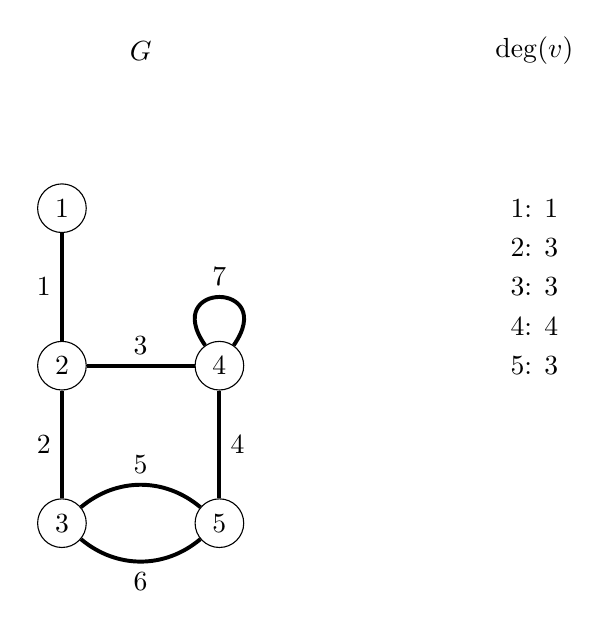
\begin{tikzpicture}
	% Define the nodes with specific positions
	\begin{scope}[xshift=0cm, yshift=0cm]
		\node (G) at (1, 6) {$G$};

		\node[circle, draw] (1) at (0, 4) {1};
		\node[circle, draw] (2) at (0, 2) {2};
		\node[circle, draw] (3) at (0, 0) {3};
		\node[circle, draw] (4) at (2, 2) {4};
		\node[circle, draw] (5) at (2, 0) {5};
	
		% Draw the edges between nodes with labels
		\draw[line width=0.5mm] (1) -- node[left] {1} (2);
		\draw[line width=0.5mm] (2) -- node[left] {2} (3);
		\draw[line width=0.5mm] (2) -- node[above] {3} (4);
		\draw[line width=0.5mm] (4) -- node[right] {4} (5);
		\draw[line width=0.5mm] (3) to[bend left=40] node[above] {5} (5);
		\draw[line width=0.5mm] (3) to[bend right=40] node[below] {6} (5);
		\draw[line width=0.5mm] (4) to[in=125,out=55,loop, min distance=1cm] node[above] {7} (4);
	\end{scope}

	% Draw the mapping from edge IDs to vertex pairs
	\begin{scope}[xshift=6cm, yshift=0cm]
		\node (E0) at (0, 6) {$\deg(v)$};
		\node (E1) at (0, 4) {1: 1};
		\node (E2) at (0, 3.5) {2: 3};
		\node (E3) at (0, 3) {3: 3};
		\node (E4) at (0, 2.5) {4: 4};
		\node (E5) at (0, 2) {5: 3};
	\end{scope}
\end{tikzpicture}
	\end{center}

	The \textit{maximum degree} of a graph $G$, denoted $\Delta(G)$, is the maximal degree of any vertex of $G$.

	A \textit{walk} of a graph $G$ is a list of edges, such that consecutive edges in the list are incident to each other.

	An \textit{$s,t$-walk} is a walk, such that the first edge is incident to the vertex $s$ and such that the last edge is incident to the vertex $t$.

	The \textit{length} of a walk is the number of edges in the walk.

	An $s,t$-walk is \textit{closed}, if $s=t$.

	A \textit{path} of a graph $G$, is a walk such that only consecutive edges of the walk are incident.

	A \textit{cycle} of a graph $G$, is a path but where the first and the last edge are incident to each other.

	A graph $G$ is \textit{connected} if there exists a $s,t$-walk for every pair of distinct vertices $s,t \in V(G)$.

	A \textit{component} of a graph, is a connected subgraph.

	A \textit{bijection} is a relation between two sets such that each element of either set is paired with exactly one element of the other set.

	A \textit{plane graph} is a drawing of a graph, such that no edges are crossing.
	
	A graph $G$ is \textit{planar}, if there exists a \textit{plane graph} of $G$.

	\begin{definition}
		(\textit{Contraction})

		A contraction is a function that given a multi-graph $G$ and pair of vertices $u,v \in V(G)$ such that $\{u,v\} \in E(G)$, then for all edges $e \in \mathbb{E}(G)$ if $\phi_G(e) = \{u,v\}$ then removes $e$ else if $\phi_G(e) = \{v,w\}$ then $\phi_G(e) = \{u,w\}$, and finally returns the resulting graph.
	\end{definition}

	\begin{center}
		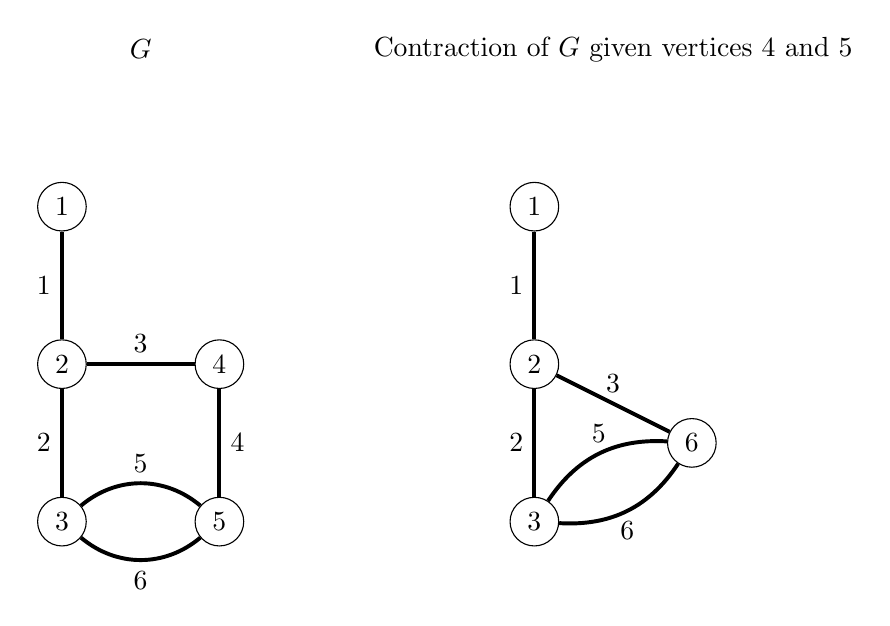
\begin{tikzpicture}
	\begin{scope}[xshift=0cm, yshift=0cm]
		\node (G) at (1, 6) {$G$};

		\node[circle, draw] (1) at (0, 4) {1};
		\node[circle, draw] (2) at (0, 2) {2};
		\node[circle, draw] (3) at (0, 0) {3};
		\node[circle, draw] (4) at (2, 2) {4};
		\node[circle, draw] (5) at (2, 0) {5};
	
		% Draw the edges between nodes with labels
		\draw[line width=0.5mm] (1) -- node[left] {1} (2);
		\draw[line width=0.5mm] (2) -- node[left] {2} (3);
		\draw[line width=0.5mm] (2) -- node[above] {3} (4);
		\draw[line width=0.5mm] (4) -- node[right] {4} (5);
		\draw[line width=0.5mm] (3) to[bend left=40] node[above] {5} (5);
		\draw[line width=0.5mm] (3) to[bend right=40] node[below] {6} (5);
	\end{scope}
	
	\begin{scope}[xshift=6cm, yshift=0cm]
		\node (G) at (1, 6) {Contraction of $G$ given vertices 4 and 5};

		\node[circle, draw] (1) at (0, 4) {1};
		\node[circle, draw] (2) at (0, 2) {2};
		\node[circle, draw] (3) at (0, 0) {3};
		\node[circle, draw] (6) at (2, 1) {6};
	
		% Draw the edges between nodes with labels
		\draw[line width=0.5mm] (1) -- node[left] {1} (2);
		\draw[line width=0.5mm] (2) -- node[left] {2} (3);
		\draw[line width=0.5mm] (2) -- node[above] {3} (6);
		\draw[line width=0.5mm] (3) to[bend left=30] node[above] {5} (6);
		\draw[line width=0.5mm] (3) to[bend right=30] node[below] {6} (6);
	\end{scope}
\end{tikzpicture}

	\end{center}
	
	\begin{definition}
		(\textit{Medial Graph})
		
		The medial graph $G^\times$ of a connected plane graph $G$ is a graph such that there is a bijection between $V(G^\times)$ and $\mathbb{E}(G)$ and such that for each face $f$ of $G$, there's an edge $e^\times \in \mathbb{E}(G^\times)$ incident to a pair of vertices $u^\times,v^\times \in V(G^\times)$ if edges $u,v \in \mathbb{E}(G)$ are consecutive in $f$.
	\end{definition}

	\begin{center}
		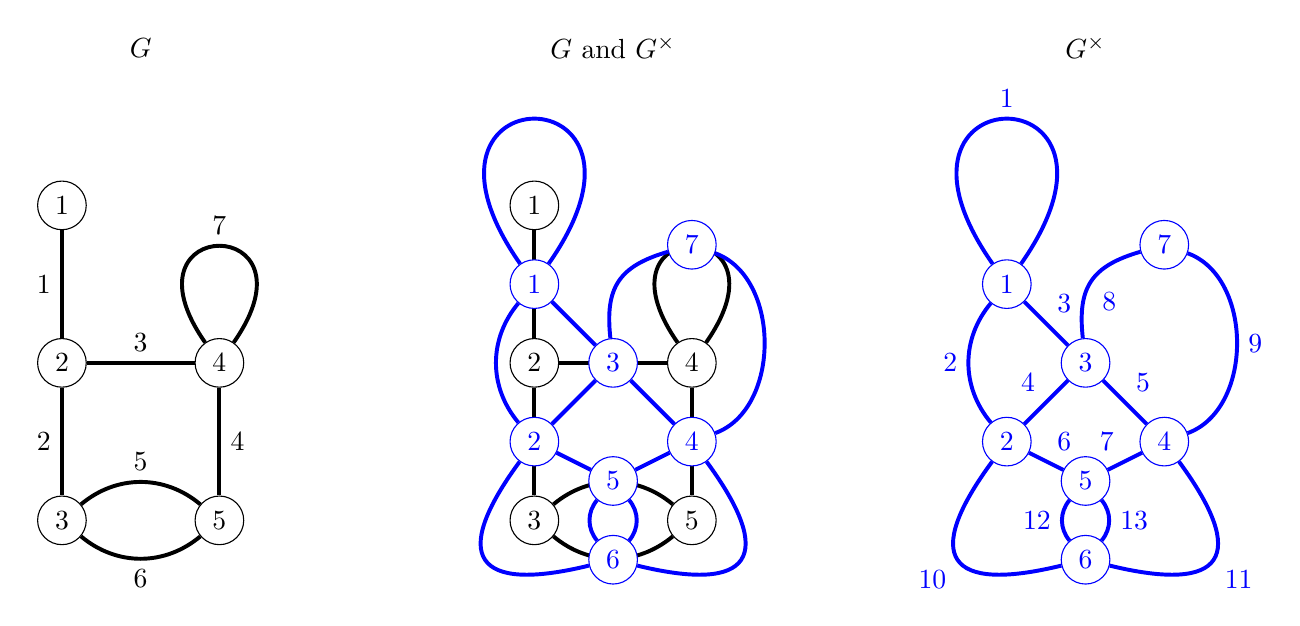
\begin{tikzpicture}
	\begin{scope}[xshift=0cm, yshift=0cm]
		\node (G) at (1, 6) {$G$};

		\node[circle, draw] (a1) at (0, 4) {1};
		\node[circle, draw] (a2) at (0, 2) {2};
		\node[circle, draw] (a3) at (0, 0) {3};
		\node[circle, draw] (a4) at (2, 2) {4};
		\node[circle, draw] (a5) at (2, 0) {5};
	
		% Draw the edges between nodes with labels
		\draw[line width=0.5mm] (a1) -- node[left] {1} (a2);
		\draw[line width=0.5mm] (a2) -- node[left] {2} (a3);
		\draw[line width=0.5mm] (a2) -- node[above] {3} (a4);
		\draw[line width=0.5mm] (a4) -- node[right] {4} (a5);
		\draw[line width=0.5mm] (a3) to[bend left=40] node[above] {5} (a5);
		\draw[line width=0.5mm] (a3) to[bend right=40] node[below] {6} (a5);
		\draw[line width=0.5mm] (a4) to[in=125,out=55,loop, min distance=2cm] node[above] {7} (a4);
	\end{scope}

	\begin{scope}[xshift=6cm, yshift=0cm]
		\node (G) at (1, 6) {$G$ and $G^\times$};

		\node[circle, draw] (a1) at (0, 4) {1};
		\node[circle, draw] (a2) at (0, 2) {2};
		\node[circle, draw] (a3) at (0, 0) {3};
		\node[circle, draw] (a4) at (2, 2) {4};
		\node[circle, draw] (a5) at (2, 0) {5};
	
		% Draw the edges between nodes with labels
		\draw[line width=0.5mm] (a1) -- (a2);
		\draw[line width=0.5mm] (a2) -- (a3);
		\draw[line width=0.5mm] (a2) -- (a4);
		\draw[line width=0.5mm] (a4) -- (a5);
		\draw[line width=0.5mm] (a3) to[bend left=40] (a5);
		\draw[line width=0.5mm] (a3) to[bend right=40] (a5);
		\draw[line width=0.5mm] (a4) to[in=125,out=55,loop, min distance=2cm] (a4);

		\node[circle, draw, color=blue, fill=white] (b1) at (0, 3) {1};
		\node[circle, draw, color=blue, fill=white] (b2) at (0, 1) {2};
		\node[circle, draw, color=blue, fill=white] (b3) at (1, 2) {3};
		\node[circle, draw, color=blue, fill=white] (b4) at (2, 1) {4};
		\node[circle, draw, color=blue, fill=white] (b5) at (1, 0.5) {5};
		\node[circle, draw, color=blue, fill=white] (b6) at (1, -0.5) {6};
		\node[circle, draw, color=blue, fill=white] (b7) at (2, 3.5) {7};
	
		% Draw the edges between nodes with labels
		\draw[line width=0.5mm, color=blue] (b1) to[in=125,out=55,loop, min distance=3cm] (b1);
		\draw[line width=0.5mm, color=blue] (b1) to[bend right=40, min distance=0.5cm] (b2);
		\draw[line width=0.5mm, color=blue] (b1) -- (b3);
		\draw[line width=0.5mm, color=blue] (b2) -- (b3);
		\draw[line width=0.5mm, color=blue] (b3) -- (b4);
		\draw[line width=0.5mm, color=blue] (b2) -- (b5);
		\draw[line width=0.5mm, color=blue] (b5) -- (b4);
		\draw[line width=0.5mm, color=blue] (b3) to[bend left=40, min distance=0.65cm] (b7);
		\draw[line width=0.5mm, color=blue] (b4) to[bend right=70, min distance=0.5cm] (b7);
		\draw[line width=0.5mm, color=blue] (b2) to[bend right=70, min distance=1.5cm] (b6);
		\draw[line width=0.5mm, color=blue] (b4) to[bend left=70, min distance=1.5cm] (b6);
		\draw[line width=0.5mm, color=blue] (b5) to[bend right=40] (b6);
		\draw[line width=0.5mm, color=blue] (b5) to[bend left=40] (b6);
	\end{scope}

	\begin{scope}[xshift=12cm, yshift=0cm]
		\node (G) at (1, 6) {$G^\times$};

		\node[circle, draw, color=blue, fill=white] (b1) at (0, 3) {1};
		\node[circle, draw, color=blue, fill=white] (b2) at (0, 1) {2};
		\node[circle, draw, color=blue, fill=white] (b3) at (1, 2) {3};
		\node[circle, draw, color=blue, fill=white] (b4) at (2, 1) {4};
		\node[circle, draw, color=blue, fill=white] (b5) at (1, 0.5) {5};
		\node[circle, draw, color=blue, fill=white] (b6) at (1, -0.5) {6};
		\node[circle, draw, color=blue, fill=white] (b7) at (2, 3.5) {7};
	
		% Draw the edges between nodes with labels
		\draw[line width=0.5mm, color=blue] (b1) to[in=125,out=55,loop, min distance=3cm] node[above] {1} (b1);
		\draw[line width=0.5mm, color=blue] (b1) to[bend right=40, min distance=0.5cm] node[left] {2} (b2);
		\draw[line width=0.5mm, color=blue] (b1) -- node[above right] {3} (b3);
		\draw[line width=0.5mm, color=blue] (b2) -- node[above left] {4} (b3);
		\draw[line width=0.5mm, color=blue] (b3) -- node[above right] {5} (b4);
		\draw[line width=0.5mm, color=blue] (b2) -- node[above right] {6} (b5);
		\draw[line width=0.5mm, color=blue] (b5) -- node[above left] {7} (b4);
		\draw[line width=0.5mm, color=blue] (b3) to[bend left=40, min distance=0.65cm] node[below right] {8} (b7);
		\draw[line width=0.5mm, color=blue] (b4) to[bend right=70, min distance=0.5cm] node[right] {9} (b7);
		\draw[line width=0.5mm, color=blue] (b2) to[bend right=70, min distance=1.5cm] node[below left] {10} (b6);
		\draw[line width=0.5mm, color=blue] (b4) to[bend left=70, min distance=1.5cm] node[below right] {11} (b6);
		\draw[line width=0.5mm, color=blue] (b5) to[bend right=40] node[left] {12} (b6);
		\draw[line width=0.5mm, color=blue] (b5) to[bend left=40] node[right] {13} (b6);
	\end{scope}
\end{tikzpicture}

	\end{center}
	
	\begin{corollary}
		A medial graph is a 4-regular plane graph.
	\end{corollary}

	\begin{definition}
		(\textit{Dual Graph})

		The dual graph $G^*$ of a plane graph $G$ is a graph with a bijection between the set of faces of $G$ and $V(G^*)$ and a bijection between $\mathbb{E}(G)$ and $\mathbb{E}(G^*)$ such that an edge $e \in \mathbb{E}(G)$ that separates two faces $f_1$,$f_2$ of $G$ is an edge $e^* \in \mathbb{E}(G^*)$ incident to $f_1^*$ and $f_2^*$.
	\end{definition}

	\begin{center}
		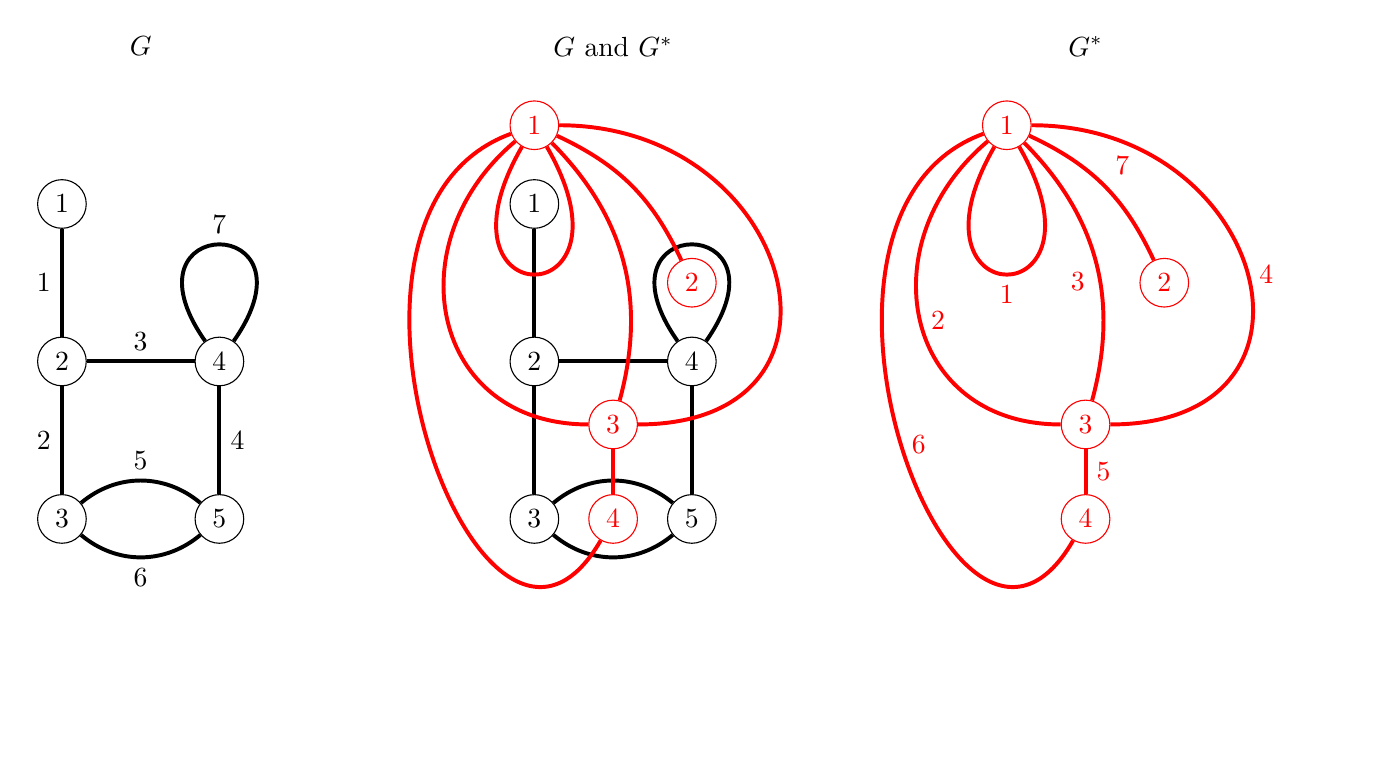
\begin{tikzpicture}
	\begin{scope}[xshift=0cm, yshift=0cm]
		\node (G) at (1, 6) {$G$};

		\node[circle, draw] (a1) at (0, 4) {1};
		\node[circle, draw] (a2) at (0, 2) {2};
		\node[circle, draw] (a3) at (0, 0) {3};
		\node[circle, draw] (a4) at (2, 2) {4};
		\node[circle, draw] (a5) at (2, 0) {5};
	
		% Draw the edges between nodes with labels
		\draw[line width=0.5mm] (a1) -- node[left] {1} (a2);
		\draw[line width=0.5mm] (a2) -- node[left] {2} (a3);
		\draw[line width=0.5mm] (a2) -- node[above] {3} (a4);
		\draw[line width=0.5mm] (a4) -- node[right] {4} (a5);
		\draw[line width=0.5mm] (a3) to[bend left=40] node[above] {5} (a5);
		\draw[line width=0.5mm] (a3) to[bend right=40] node[below] {6} (a5);
		\draw[line width=0.5mm] (a4) to[in=125,out=55,loop, min distance=2cm] node[above] {7} (a4);
	\end{scope}

	\begin{scope}[xshift=6cm, yshift=0cm]
		\node (G) at (1, 6) {$G$ and $G^*$};

		\node[circle, draw] (a1) at (0, 4) {1};
		\node[circle, draw] (a2) at (0, 2) {2};
		\node[circle, draw] (a3) at (0, 0) {3};
		\node[circle, draw] (a4) at (2, 2) {4};
		\node[circle, draw] (a5) at (2, 0) {5};
	
		% Draw the edges between nodes with labels
		\draw[line width=0.5mm] (a1) -- (a2);
		\draw[line width=0.5mm] (a2) -- (a3);
		\draw[line width=0.5mm] (a2) -- (a4);
		\draw[line width=0.5mm] (a4) -- (a5);
		\draw[line width=0.5mm] (a3) to[bend left=40] (a5);
		\draw[line width=0.5mm] (a3) to[bend right=40] (a5);
		\draw[line width=0.5mm] (a4) to[in=125,out=55,loop, min distance=2cm] (a4);

		\node[circle, draw, color=red, fill=white] (d1) at (0, 5) {1};
		\node[circle, draw, color=red, fill=white] (d2) at (2, 3) {2};
		\node[circle, draw, color=red, fill=white] (d3) at (1, 1.2) {3};
		\node[circle, draw, color=red, fill=white] (d4) at (1, 0) {4};
		
		\draw[line width=0.5mm, color=red] (d1) to[in=240, out=300, loop, min distance=2.5cm] (d1);
		\draw[line width=0.5mm, color=red] (d1) to[bend left=20] (d2);
		\draw[line width=0.5mm, color=red] (d1) to[bend left=30] (d3);
		\draw[line width=0.5mm, color=red] (d1) to[in=180, out=220, min distance=2cm] (d3);
		\draw[line width=0.5mm, color=red] (d1) to[in=0, out=0, min distance=3cm] (d3);
		\draw[line width=0.5mm, color=red] (d3) -- (d4);
		\draw[line width=0.5mm, color=red] (d1) to[in=240, out=200, min distance=3cm] (d4);
	\end{scope}

	\begin{scope}[xshift=12cm, yshift=0cm]
		\node (G) at (1, 6) {$G^*$};

		\node[circle, draw, color=red, fill=white] (d1) at (0, 5) {1};
		\node[circle, draw, color=red, fill=white] (d2) at (2, 3) {2};
		\node[circle, draw, color=red, fill=white] (d3) at (1, 1.2) {3};
		\node[circle, draw, color=red, fill=white] (d4) at (1, 0) {4};
		
		\draw[line width=0.5mm, color=red] (d1) to[in=240, out=300, loop, min distance=2.5cm] node[below] {1} (d1);
		\draw[line width=0.5mm, color=red] (d1) to[in=180, out=220, min distance=2cm] node[right] {2} (d3);
		\draw[line width=0.5mm, color=red] (d1) to[bend left=30] node[below left] {3} (d3);
		\draw[line width=0.5mm, color=red] (d1) to[in=0, out=0, min distance=3cm] node[right] {4} (d3);
		\draw[line width=0.5mm, color=red] (d3) to node[right] {5} (d4);
		\draw[line width=0.5mm, color=red] (d1) to[in=240, out=200, min distance=3cm] node[right] {6} (d4);
		\draw[line width=0.5mm, color=red] (d1) to[bend left=20] node[above right] {7} (d2);
	\end{scope}
\end{tikzpicture}

	\end{center}

	A \textit{tree} is a connected graph with no cycles.

	A \textit{leaf} $v$ of a tree $T$, is a vertex $v \in V(T)$ of degree 1.

	An \textit{internal vertex} $v$ of a tree $T$, is a vertex $v \in V(T)$ of degree at least 2.

	Let the \textit{leaf set} of a tree $T$, denoted $L(T)$, be the set of all vertices of $T$ that are also leaves.

	A \textit{Branch Decomposition} $(B_G, \delta_G)$ of a graph $G$ consists of firstly, a tree $B_G$ where every internal vertex of $B_G$ has degree 3; in other words, $B_G$ is an unrooted binary tree, and secondly a bijection $\delta_G$ between $\mathbb{E}(G)$ and $L(B_G)$.

	Removing any edge $e \in \mathbb{E}(B_G)$ partitions $B_G$ into 2 trees $P_e$ and $Q_e$. The set $L(P_e) \cap L(Q_e)$ is called a \textit{middle set} of $B_G$ given $e$, denoted $Z(B_G,e)$. The maximal cardinality of any middle set of $B_G$ given any $e$ of $B_G$ is the width of $B_G$; in other words, the width of $B_G$ is $\max\{ |Z(B, e)| \st e \in \mathbb{E}(B) \}$.

	There might exist many branch decompositions of a graph $G$.

	A \textit{Minimal Branch Decomposition} of $G$ is any branch decomposition of $G$ of minimal width among all branch decompositions of $G$.

	A \textit{Carving Decomposition} $(C_G, \lambda_G)$ of a graph $G$ consists of firstly, a tree unrooted binary tree $C_G$ and secondly a bijection $\lambda_G$ between $V(G)$ and $L(C_G)$.

	Removing any edge $e \in \mathbb{E}(C_G)$ partitions $C_G$ into 2 trees $P_e$ and $Q_e$. The set $L(P_e) \cap L(Q_e)$ is called a \textit{middle set} of $C_G$ given $e$, denoted $Z(C_G,e)$. The maximal cardinality of any middle set of $C_G$ given any $e$ of $C_G$ is the width of $C_G$; in other words, the width of $C_G$ is $\max\{ |Z(C_G, e)| \st e \in \mathbb{E}(C_G) \}$.

	There might exist many carving decompositions of a graph $G$.

	A \textit{Minimal Carving Decomposition} of $G$ is any carving decomposition of $G$ of minimal width among all carving decompositions of $G$.

\section{Description of the problem}

	The main computational problem of this paper is \textsc{The Planar Minimal Branch Decomposition Problem}.

	\begin{definition}
		\textsc{The Planar Minimal Branch Decomposition Problem}

		Input: Given a simple connected planar graph $G$.

		Output: A minimal branch decomposition of $G$.
	\end{definition}

	Here are some informal definitions to unpack the aforementioned properties of graphs.

	\begin{definition}\label{def:mbdp}
		\textsc{The Minimal Branch Decomposition Problem}

		Input: Given a simple connected graph $G$.

		Output: A minimal branch decomposition of $G$.
	\end{definition}

	The algorithm described in this paper solves \textsc{The Planar Minimal Branch Decomposition Problem}, which can be computed in polynomial time.

	The width of a minimal branch decomposition of $G$ is called the branch width of $G$.

\section{The algorithm}
	This section describes the algorithm given by Seymour and Thomas\cite{ST93} by identifying a set of practical problems and subproblems and how they relate.
	
	Problem \ref{def:mbdp} is the overarching problem, and can be broken down into many smaller subproblems.

	Considering a graph $G$, you can compute a minimal branch decomposition $(B_G, \delta_G)$ of $G$ from a minimal carving decomposition $(C_{G^\times}, \lambda_{G^\times})$ of the medial graph $G^\times$ of $G$. Do this by replacing the vertices in leaves of the carving decomposition with edges, using the mapping between edges and vertices from computing the medial graph; 

	Therefore problem \ref{def:mbdp} break down into problems \ref{problem:mcd-to-mbd}, \ref{problem:medial} and \ref{problem:mcd}.

	\begin{problem}\label{problem:mcd-to-mbd}
		Given a minimal carving decomposition of a medial graph of $G$, output a minimal branch decomposition of $G$.
	\end{problem}

	\begin{problem}\label{problem:medial}
		Given a graph $G$, output a medial graph and a bijectional mapping between medial nodes and vertex pairs.
	\end{problem}

	\begin{problem}\label{problem:mcd}
		Given a plane graph $M$ and function to compute the carving width of a graph, output a minimal carving decomposition of $M$.
	\end{problem}

	Implementing a function to solve \ref{problem:mcd-to-mbd} is described in \ref{impl:mcd-to-mbd}.

	To solve \ref{problem:medial} is a matter of following the definition.

	I will refer to vertices and edges of the medial graph as "nodes" and "links" in an attempt at disambiguation. 

	Computing a medial graph is described in \ref{impl:medial}.

	To solve \ref{problem:mcd} \ref{} gives a contraction algorithm.

	Doing a series of edge contractions (contraction of all edges incident to a pair of vertices) on a graph $M$, where the carving width does not increase until 3 vertices remain, then the series of contracted edges along with the three vertices can be assembled into a minimal carving decomposition of $M$.
	
	I will defer describing exactly how to assemble a minimal carving decomposition to \ref{impl:mcd}.

	The contraction algorithm depends on a function to compute a contraction and a function to compute the carving width. This is problems \ref{problem:contraction} and \ref{problem:cw}.

	\begin{problem}\label{problem:contraction}
		Given a graph $M$ and a pair of vertices $\{u, v\}$, output a graph resulting from a contraction of all edges incident to $u$ and $v$ if $u$ and $v$ are neighbors.
	\end{problem}

	\begin{problem}\label{problem:cw}
		Given a plane graph $M$ that might have parallel edges, output the carving width of $M$.
	\end{problem}

	First consider problem \ref{problem:contraction}.

	Informally; a contraction is merging two vertices into one and letting incident edges connect to the new vertex. The contraction in this paper differs a bit from conventional definitions of edge- and vertex-contractions, as other definitions might result in self-loops when contracting one of multiple parallel edges.


	Computing a medial graph is described in \ref{impl:medial}.

	Now consider problem \ref{problem:cw}.

	The rat-catching algorithm decides $cw(M) \geq k$ with $k$ being in the positive integers. This is a monotonic boolean space, so you can perform a binary search to find the smallest $k$ where $cw(M) \geq k$ is true.

	The rat-catching algorithm can be described as a game of two players, the rat and rat-catcher. Considering a graph $M$, the edges of a face can be thought of as walls of a room and vertices as the corners of some rooms. The rat moves from corner to corner along the walls and the rat-catcher moves from room to room through some wall. The rat-catcher can force the rat away from some walls by making noise. A round of this game is played with some noise level $k$. The rat-catcher wins if they can force the rat to be in some wall of the room that they are in, with noise level $k$, and the rat wins if there is a strategy whereby the rat can escape indefinitely.

	Additionally, if $\Delta(M) \geq k$ then the rat wins. The argument for why this is true is glossed over in \ref{BGZ15}. This is discussed in section \ref{}.

	So assuming $\Delta(M) < k$ the game is played.

	For some noise level and location of the rat-catcher, exactly which edges are noisy and which are quiet are definitions \ref{def:edge-quiet} and \ref{def:face-quiet}.

	An edge $e$ is called quiet iff. $e$ is not noisy.

	\begin{definition}\label{def:edge-quiet}
		When the rat-catcher is on some edge $e_1$, then edge $e_2$ is noisy iff. there is a closed walk of length scrictly less than $k$ containing $e_1^*$ and $e_2^*$ in the dual $M^*$.
	\end{definition}

	\begin{definition}\label{def:face-quiet}
		When the rat-catcher is on some room $f$, then edge $e$ is noisy iff. there is a closed walk of length scrictly less than $k$ containing $f^*$ and $e^*$ in the dual $M^*$.
	\end{definition}

	A quiet subgraph $Q(M, k, e)$, for some graph $M$, some noise level $k$ and some $e \in \mathbb{E}(M)$, is a subgraph of $M$ with $V(Q(M, k, e)) = V(M)$ and

	$\mathbb{E}(Q(M, k, e)) = \{e_1 \st $ every closed walk of $M^*$ containing $e_1^*$ and $e_2^*$ has length at least $k\}$

	\begin{problem}\label{problem:noisy-subgraph}
		Given a plane graph $M$ that might have parallel edges, an edge $e \in \mathbb{E}(M)$, and noise level $k \in \mathbb{N}$, output the quiet subgraph $Q(M, k, e)$.
	\end{problem}

	Problem \ref{problem:noisy-subgraph} depends on a function for computing the dual of a graph. Computing a dual graph is problem \ref{problem:dual}.

	\begin{problem}\label{problem:dual}
		Given a plane graph $M = \{V, E\}$ that might have parallel edges, output the dual of $M$.
	\end{problem}

	The game states and possible moves, for some graph $M$ and some noise level $k$, can be described as a graph $H(M, k)$.

	Let $F(M)$ be the set of faces of $M$.

	Let $S$ be every possible state when the rat-catcher is in a face some of which might be losing states. $S = \{ (f, v) \st v \in V(M) \land f$ is a face of $ M \}$.

	Let $T$ be every possible state when the rat-catcher is on an edge. $T = \{ (e, C) \st e \in \mathbb{E}(M) \land C$ is a component of $Q(M, k, e) \}$.

	Computing the quiet subgraph requires the dual graph. 
	
	With the graph $H$, the only missing piece of the rat-catching algorithm is how to determine the outcome.

	You can mark states of the graph $H$ that are losing states, and then repeatedly mark any state that leads to a losing state, until either every state is marked or no more states can be marked. If every state is marked then the rat-catcher wins, otherwise the rat wins.

\section{The implementation}

	For the upcoming problems one needs to deal with parallel edges and be able to tell them apart, therefore the implementation uses a data structure that encapsulates an adjacency list of edges and a map from unique edge ids its vertexpair.

	I have chosen to assign IDs such that if one half-edge has ID $i$ then the other half-edge has ID $-i$, therefore the absolute value $|i|$ uniquely identifies an undirected edge.

	\pyfile{graph.py}{0}{100}

	\subsection{Computing a minimal branch decomposition}\label{impl:mcd-to-mbd}
		
		Solving problem \ref{problem:mcd-to-mbd}.

		For both branch- and carving-decompositions, I have chosen a data structure of tuples of tuples or integers. This has a straightforward translation to the Newick tree format, a concise notation for tree structures.

		To then solve the above-mentioned problem, the implementation recursively returns a copy of any tuple, but returns a tuple of integers for any integer, using the mapping from medial node to vertex pair.

		\pyfile{branch_decomposition.py}{5}{19}
		
	\subsection{Computing a medial graph}\label{impl:medial}
		
		Solving problem \ref{problem:medial}.

		I assume that the input graph $G$ is a rotation system of a planar graph; an adjacency list such that the neighborhoods are given in clockwise ordering according to some plane embedding of $G$.
		
		Given this format, any two consecutive edges $e_1$ and $e_2$ in some face of $G$ are therefore consecutive vertices in the neighborhood of the vertex that $e_1$ and $e_2$ share.

		The implementation adds all medial links around some vertex for each vertex in $G$. 
		
		The clockwise ordering of neighborhoods of $G$ becomes counterclockwise ordering of neighborhoods of the medial $M$. The medial graph of a plane graph is 4-regular \ref{}. From the perspective of some medial node $v$, in some single iteration of the loop on line 14, two links are added to the neighborhood of $v$ in counterclockwise ordering, and later the two other links are added to the neighborhood of $v$ also in counterclockwise ordering.
		
		\pyfile{medial_graph.py}{4}{22}
	
	\subsection{Computing a minimal carving decomposition}\label{impl:mcd}

		Solving problem \ref{problem:mcd}.

		The implementation finds a nonincreasing contraction by doing a linear search over every edge. No consideration has yet been given to any potential clever orderings of the edges that might improve the running time.

		The sequence of contracted edges is found and reassembled into a minimal carving decomposition.

		The "contraction" function returns a new unique vertex ID, therefore by saving which vertex is a contraction of which vertex pair in the "edges" dictionary, constructing the decomposition is then a matter of recursively expanding any vertices that were a result of a contraction into a tuple of the vertex pair that is was composed of. Repeating this until all only vertices of $M$ remain gives a carving decomposition in Newick-like nested tuple format.

		\pyfile{carving_decomposition.py}{8}{48}

	\subsection{Contraction}\label{impl:contraction}

		Solving problem \ref{problem:contraction}.

		As the resulting graph is later given as an argument to functions assuming a rotation system of a planar graph, the implementation needs to preserve this invariant when contracting.

		As this contraction is a contraction of ALL edges connecting a pair of vertices, the resulting graph will not exhibit any self-loops. I suspect reconciling this and the rotation system could be difficult, but luckily in this context, it is irrelevant.

		For a contraction of vertices $a$ and $b$, I have chosen to create a new vertex ID $c$ instead of reusing $a$ or $b$ as this later makes assembling the carving decomposition easier.

		First, update any edges incident to either $a$ or $b$. Then creating the neighborhood of the new vertex $c$ from the contraction of vertices $a$ and $b$, is done by firstly finding any shared edge $e$. In this implementation the first shared edge $e$ in the neighborhood of $a$. This edge has some ID $e$ and the other half-edge with ID $-e$ will therefore be in the neighborhood of $b$. Now  "rotating" the neighborhoods of $a$ and $b$ such edge $e$ and $-e$ is at index 0 in both lists means that a concatenation of the lists will preserve the ordering around the new vertex $c$. And finally, remove any edges connecting $a$ and $b$.
		
		This is where telling apart parallel edges, which the Graph class allows, becomes very useful. Inferring where to stitch together the neighborhoods to preserve the ordering, just from a normal adjacency list, becomes a way harder problem.

		\pyfile{contraction.py}{4}{49}

	\subsection{Carving width and the rat cathing algorithm}\label{impl:cw}

		Solving problem \ref{problem:cw}

		The vertices of the game state graph $H$ are initialized by computing the elements of $T$ and $S$, while edges of $H$ are not explicitly kept in any data structure, but instead checked while playing the game.

		Losing states - the tuples $(f,v) \in S$ where $v \in f$ - are marked as losing.

		The outcome of the game is computed by marking states as losing.
		
		Considering a tuple $(e, C) \in T$, if all $(f, v)$ where $v \in V(C)$ is losing then $(e, C)$ is losing.

		Considering a tuple $(f, v)$, if there exists a tuple $(e, C)$ that is losing where $e \in f$ and $v \in V(C)$ then $(f, v)$ is losing.

		\pyfile{carving_width.py}{7}{9}
		\pyfile{carving_width.py}{78}{130}

	\subsection{Quiet subgraph}\label{impl:quiet}

		Solving problem \ref{problem:noisy-subgraph}.

		Using definition \ref{def:edge-quiet}: When the rat-catcher is on some edge $e_1$, then edge $e_2$ is noisy iff. there is a closed walk of length scrictly less than $k$ containing $e_1^*$ and $e_2^*$ in the dual $M^*$.

		Let $s_1$ and $t_1$ be the vertex pair for the link $e_1^*$ and let $s_2$ and $t_2$ be the vertex pair for the link $e_2^*$.

		\begin{claim}
			The shortest closed walk that includes both $e_1^*$ and $e_2^*$ has the same length as either $$d(s_1, s_2) + d(t_1, t_2) + 2$$ or $$d(s_1, t_1) + d(s_2, t_2) + 2$$. Where $d(u, v)$ is the length of the shortest $u,v$-path.
		\end{claim}

		The single source shortest distances can then be computed using a breadth-first approach.

		Using the mapping from links to edges, and the fact that an edge $e$ is called quiet iff. $e$ is not noisy, the quiet edges can be obtained in the natural way.

		Computing the quiet subgraph and the components thereof is done with a depth-first search approach.

		The edges of the components are irrelevant for the rest of the algorithm, so only a list of vertices is returned for each component.

		\pyfile{carving_width.py}{10}{76}

	\subsection{Dual graph}\label{impl:dual}

		Solving problem \ref{problem:dual}

		No other path of the implementation needs the assumption that the dual is planar, therefore no clockwise or counterclockwise ordering of the neighborhoods of the adjacency list is needed.

		The dual has a vertex for each face of the input graph. The faces are found by selecting an unmarked half-edge, and then marking all the edges of the face it belongs to, by following the edges that are just next to each other in the ordered neighborhoods.

		% https://en.wikipedia.org/wiki/Rotation_system

		The next halfedge $e_{i+1}$ after the current halfedge $e_i = \{u, v\}$ is the edge just before $-e_i$ in the ordered neighborhood around $v$.

		\pyfile{dual_graph.py}{21}{22}

		\pyfile{dual_graph.py}{4}{50}

\newpage
\section{References}
	\printbibliography

\newpage
\section{Appendix}
	\pyfile{branch_decomposition.py}{0}{1000}
	\pyfile{branch_width_brute_force.py}{0}{1000}	
	\pyfile{branch_width.py}{0}{1000}
	\pyfile{carving_decomposition.py}{0}{1000}
	\pyfile{carving_width_brute_force.py}{0}{1000}
	\pyfile{carving_width.py}{0}{1000}
	\pyfile{contraction.py}{0}{1000}
	\pyfile{dual_graph.py}{0}{1000}
	\pyfile{Graph.py}{0}{1000}
	\pyfile{medial_graph.py}{0}{1000}
	\pyfile{parse_graph.py}{0}{1000}
	\pyfile{parse_newick.py}{0}{1000}

\end{document}
